\chapter{Tulevaisuus\label{tulevaisuus}}

Tutkielman lopuksi pohditaan kirjautumismenetelmien tulevaisuutta. Mikä on nykyisten kirjautumismenetelmien tulevaisuus. Mitä mahdollisia uusia kirjautumismenetelmiä tulevaisuudessa saatetaan kehittää ja käyttää.

\begin{figure}[ht]
    \centering
    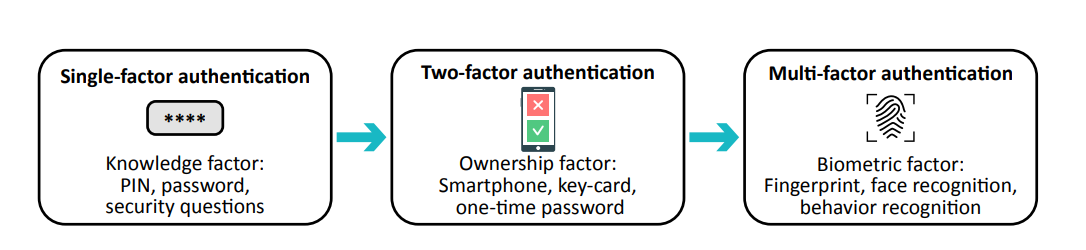
\includegraphics[width=12cm]{template/figures/Evolution-of-authentication-methods.PNG}
    \caption{Kirjautumismenetelmien kehitys \citep{cryptography2010001}}
    \label{fig:authentication-evolution}
\end{figure}

Kuva \ref{fig:authentication-evolution} havainnollistaa varmentamismenetelmien kehityksen yksivaiheisesta varmentamisesta monivaiheiseen varmentamiseen. Kuvan \ref{fig:authentication-evolution} ensimmäinen vaihe on yksivaiheinen varmentaminen. Tästä seuraava askel on kaksivaiheinen varmentaminen. Ja kolmas askel on monivaiheinen todentaminen. 

Biometristen varmentamismenetelmissä saatetaan nähdä kehitystä ja uusia menetelmiä tulevaisuudessa
EKG signaalin käyttäminen biometrisessä varmentamisessa on yksi mahdollinen tulevaisuuden vaihtoehto. Varmentaminen perustuu EKG signaaliin, joka on yksilöllinen. EKG signaalin käyttämisestä tekee mielenkiintoisen se, että sen kopiointi tai manipulointi on lähes mahdotonta. EKG:tä voisi olla mahdollinen biometrinen varmentamismenetelmä. \citep{shdefat2018utilizing}
Monivaiheinen biometrinen varmentaminen on mahdollinen tulevaisuuden varmentamismenetelmä. Menetelmä perustuisi kahteen tai useampaan biometriseen tunnistuksen. Tämän avulla pystyttäisiin tunnistamaan ja varmentamaan henkilöllisyys paremmin. \citep{biometric_authentication_systems}

Passiivista biometrista dataa käyttäminen varmentamisessa olisi myös mahdollista. Passiivinen biometrinen todentaminen on aktiivisen biometrisen todentamisen vastakohta. Se ei vaadi käyttäjän panosta esimerkiksi sormen laittamista laitteeseen, joka lukee sormenjäljen. Passiivista biometrista dataa voi olla esimerkiksi henkilön tapa kävellä, millä tavalla pitää ja käyttää puhelinta, millä tavalla puhuu, kehon lämpötila, kehon ääriviivat. Nykyään käytössä oleva kasvojen tunnistaminen voidaan laskea passiiviseksi tunnistamiseksi. Se ei vaadi käyttäjältä panosta varmentamiseen. \citep{biometric_authentication_systems}\citep{passive_biometrics}

